\pagestyle{plain}
\backgroundsetup{contents=,color=red!30}
\pagecolor{white}

% \begin{center}
%     \color{red!50!white}
%     \textbf{\huge{STATUT - \documentStatus}}
% \end{center}

\vfill


\color{black}
\begin{center}
    % \includegraphics[width=0.5\linewidth]{images/logos/fib.png} \\
    
\includegraphics[height=2cm]{images/logos/upc_logo.jpeg} \\
    \vfill
    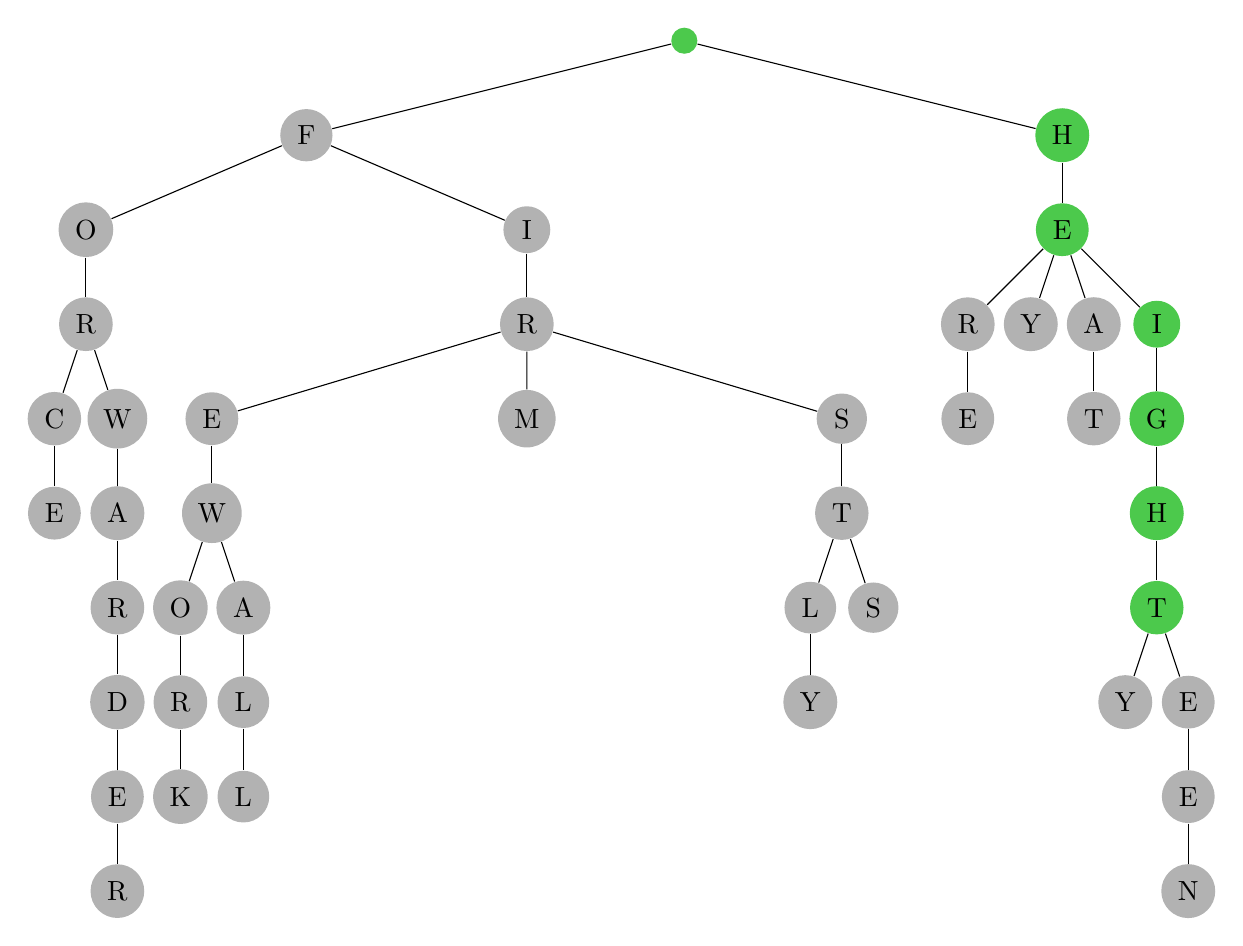
\begin{tikzpicture}[scale=0.8]
\node [circle, fill=green!70!black!70]{}[sibling distance=12cm]
	child{node[circle, fill=black!30]{F}[sibling distance=7cm]
		child{node[circle, fill=black!30]{O}[sibling distance=1cm]
			child{node[circle, fill=black!30]{R}[sibling distance=1cm]
				child{node[circle, fill=black!30]{C}[sibling distance=1cm]
					child{node[circle, fill=black!30]{E}[sibling distance=1cm]
					}
				}
				child{node[circle, fill=black!30]{W}[sibling distance=1cm]
					child{node[circle, fill=black!30]{A}[sibling distance=1cm]
						child{node[circle, fill=black!30]{R}[sibling distance=1cm]
							child{node[circle, fill=black!30]{D}[sibling distance=1cm]
								child{node[circle, fill=black!30]{E}[sibling distance=1cm]
									child{node[circle, fill=black!30]{R}[sibling distance=1cm]
									}
								}
							}
						}
					}
				}
			}
		}
		child{node[circle, fill=black!30]{I}[sibling distance=1cm]
			child{node[circle, fill=black!30]{R}[sibling distance=5cm]
				child{node[circle, fill=black!30]{E}[sibling distance=1cm]
					child{node[circle, fill=black!30]{W}[sibling distance=1cm]
						child{node[circle, fill=black!30]{O}[sibling distance=1cm]
							child{node[circle, fill=black!30]{R}[sibling distance=1cm]
								child{node[circle, fill=black!30]{K}[sibling distance=1cm]
								}
							}
						}
						child{node[circle, fill=black!30]{A}[sibling distance=1cm]
							child{node[circle, fill=black!30]{L}[sibling distance=1cm]
								child{node[circle, fill=black!30]{L}[sibling distance=1cm]
								}
							}
						}
					}
				}
				child{node[circle, fill=black!30]{M}[sibling distance=1cm]
				}
				child{node[circle, fill=black!30]{S}[sibling distance=1cm]
					child{node[circle, fill=black!30]{T}[sibling distance=1cm]
						child{node[circle, fill=black!30]{L}[sibling distance=1cm]
							child{node[circle, fill=black!30]{Y}[sibling distance=1cm]
							}
						}
						child{node[circle, fill=black!30]{S}[sibling distance=1cm]
						}
					}
				}
			}
		}
	}
	child{node[circle, fill=green!70!black!70]{H}[sibling distance=1cm]
		child{node[circle, fill=green!70!black!70]{E}[sibling distance=1cm]
			child{node[circle, fill=black!30]{R}[sibling distance=1cm]
				child{node[circle, fill=black!30]{E}[sibling distance=1cm]
				}
			}
			child{node[circle, fill=black!30]{Y}[sibling distance=1cm]
			}
			child{node[circle, fill=black!30]{A}[sibling distance=1cm]
				child{node[circle, fill=black!30]{T}[sibling distance=1cm]
				}
			}
			child{node[circle, fill=green!70!black!70]{I}[sibling distance=1cm]
				child{node[circle, fill=green!70!black!70]{G}[sibling distance=1cm]
					child{node[circle, fill=green!70!black!70]{H}[sibling distance=1cm]
						child{node[circle, fill=green!70!black!70]{T}[sibling distance=1cm]
							child{node[circle, fill=black!30]{Y}[sibling distance=1cm]
							}
							child{node[circle, fill=black!30]{E}[sibling distance=1cm]
								child{node[circle, fill=black!30]{E}[sibling distance=1cm]
									child{node[circle, fill=black!30]{N}[sibling distance=1cm]
									}
								}
							}
						}
					}
				}
			}
		}
	}
;
\end{tikzpicture}


    \vfill
    \rule{\linewidth}{0.5mm} \\[1cm]
    {\Huge \textsc{\textcolor{fib_red}{Word Games}}}\\[1cm]
    {\Large \textsc{Assignment}}\\[0.4cm]
    {\huge \textsc{\textbf{Advanced data structures}}}\\[1cm]
    {\Large \textsc{Master in Research and Innovation - UPC}}\\[0.4cm]
    \rule{\linewidth}{0.5mm} \\[1.5cm]
\end{center}

\vfill

\textbf{Author:}
\begin{itemize}
\item Pierre \textsc{Jézégou}\newline
\textit{(Engineering student at École Centrale de Lille, Exchange student at UPC)}
\end{itemize}

\newpage
\color{black}
\pagecolor{white}
\pagestyle{fancy}